\chapter{Demonstration slides}\label{demo-slides}

\begin{figure}
    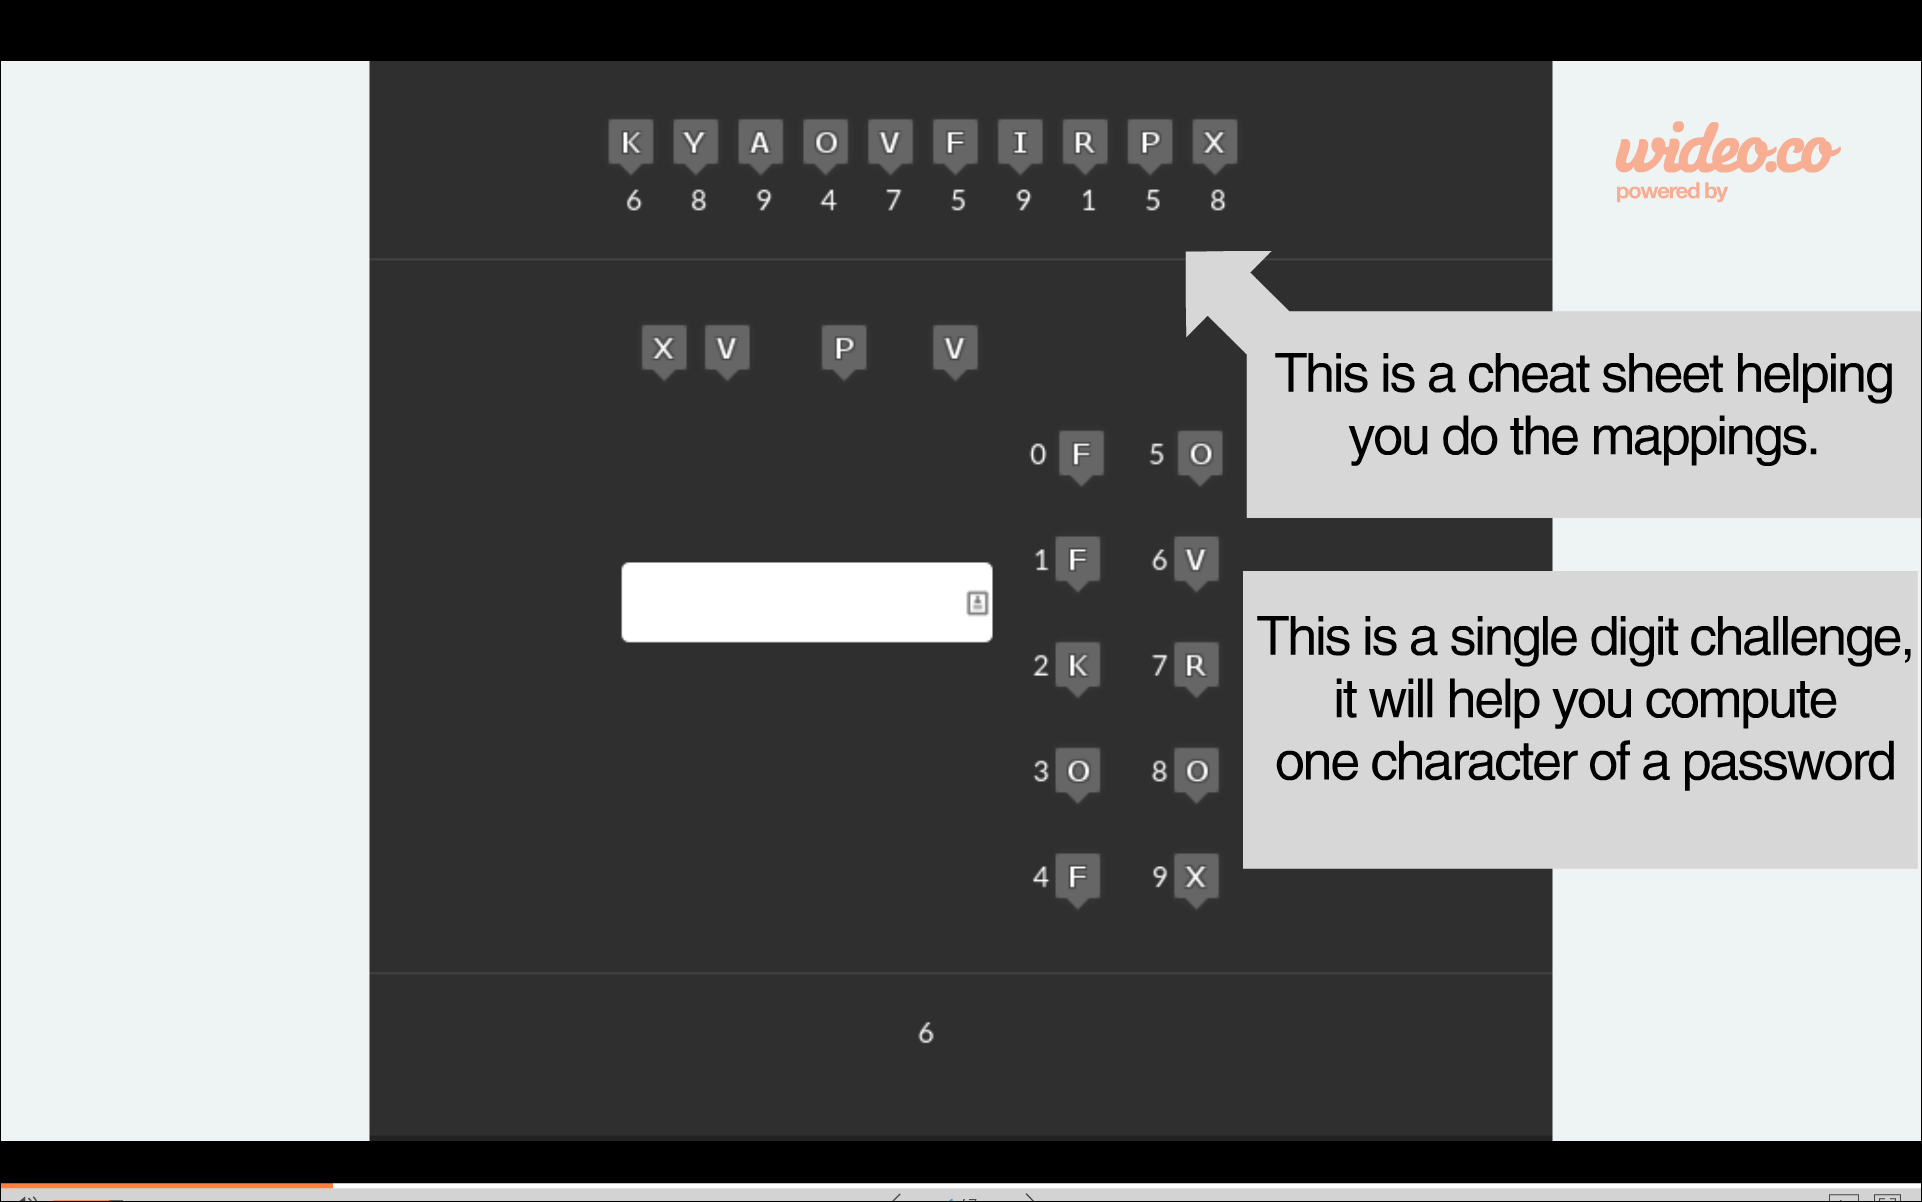
\includegraphics[width=\textwidth]{slides/slide1}
    \caption{Demo slide 1.}
    \label{slide1}
\end{figure}


\begin{figure}
    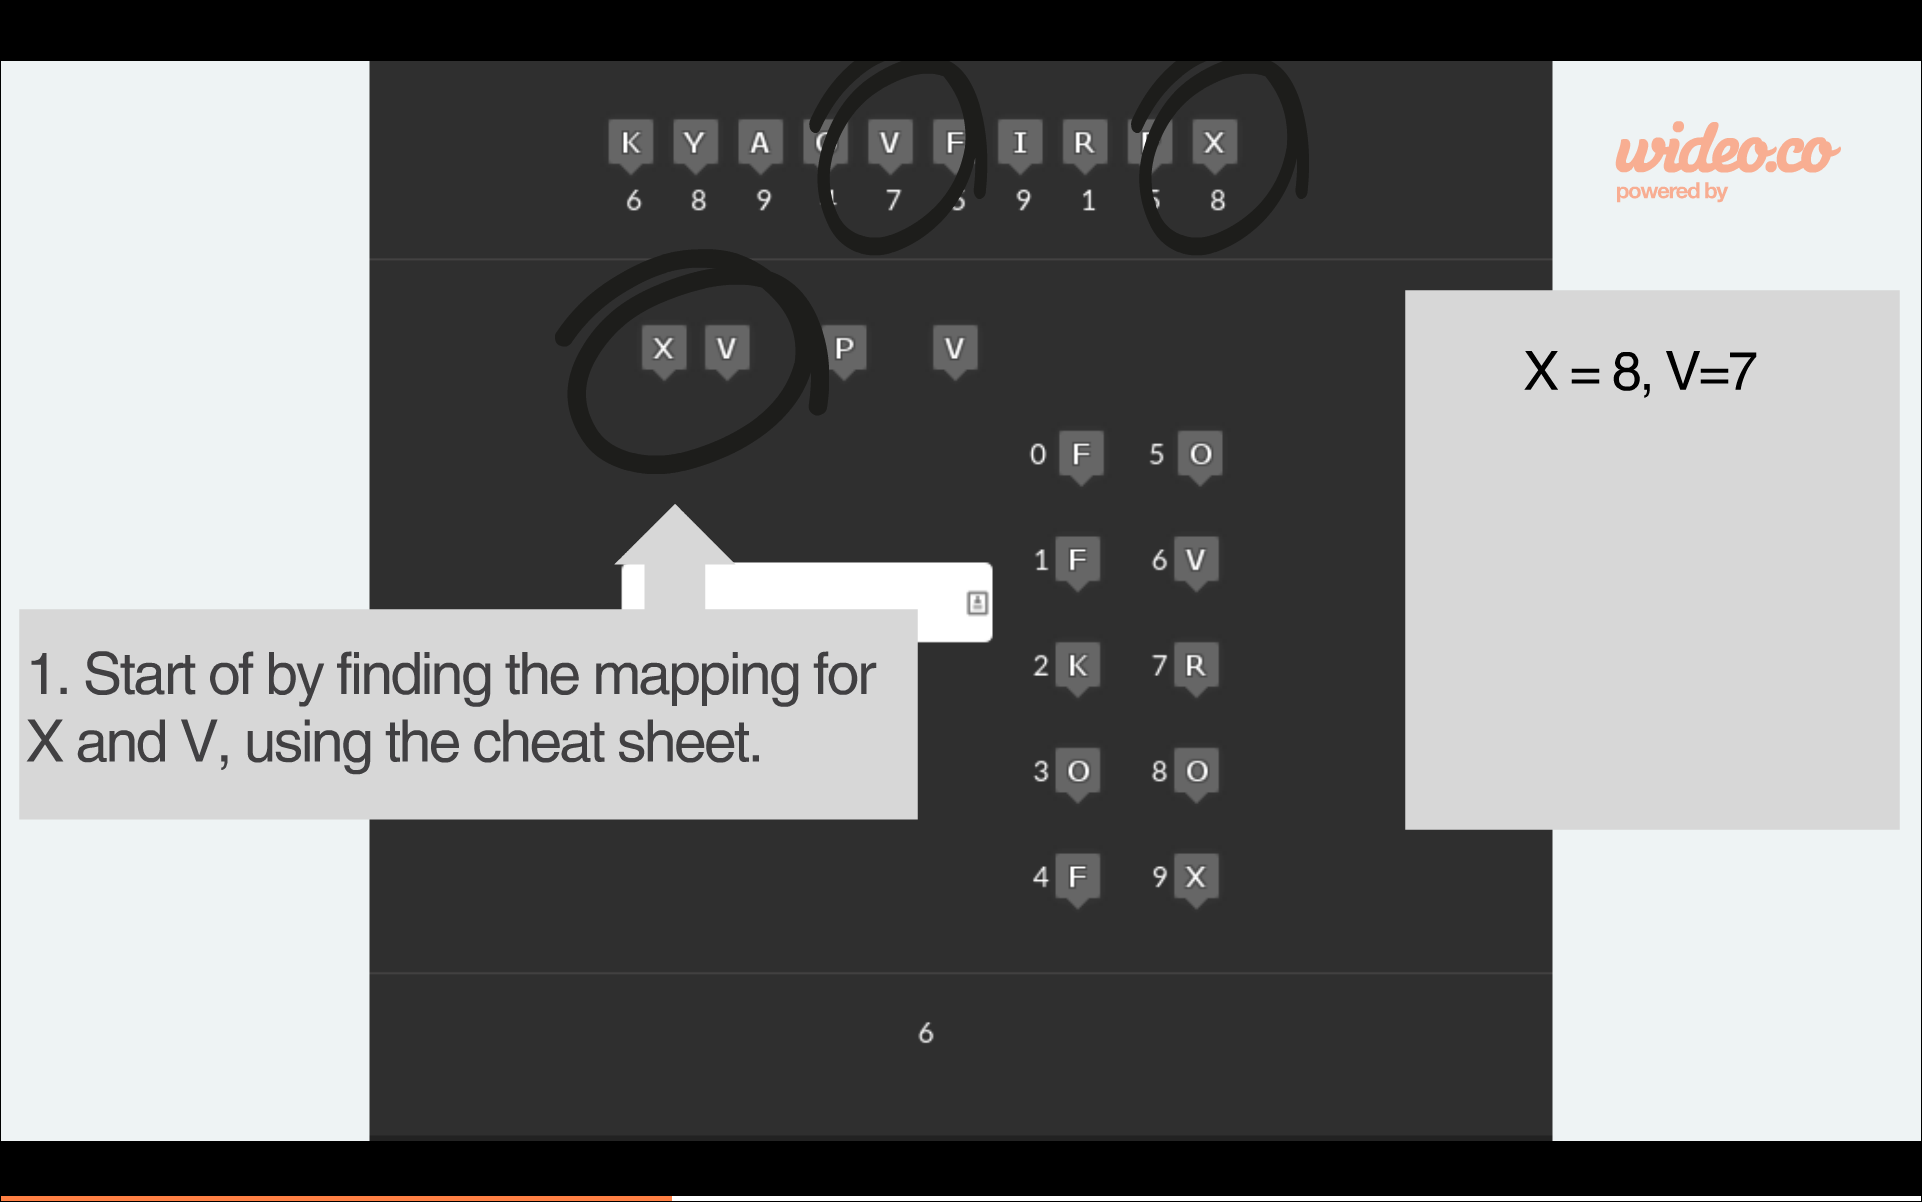
\includegraphics[width=\textwidth]{slides/slide2}
    \caption{Demo slide 2.}
    \label{slide2}
\end{figure}


\begin{figure}
    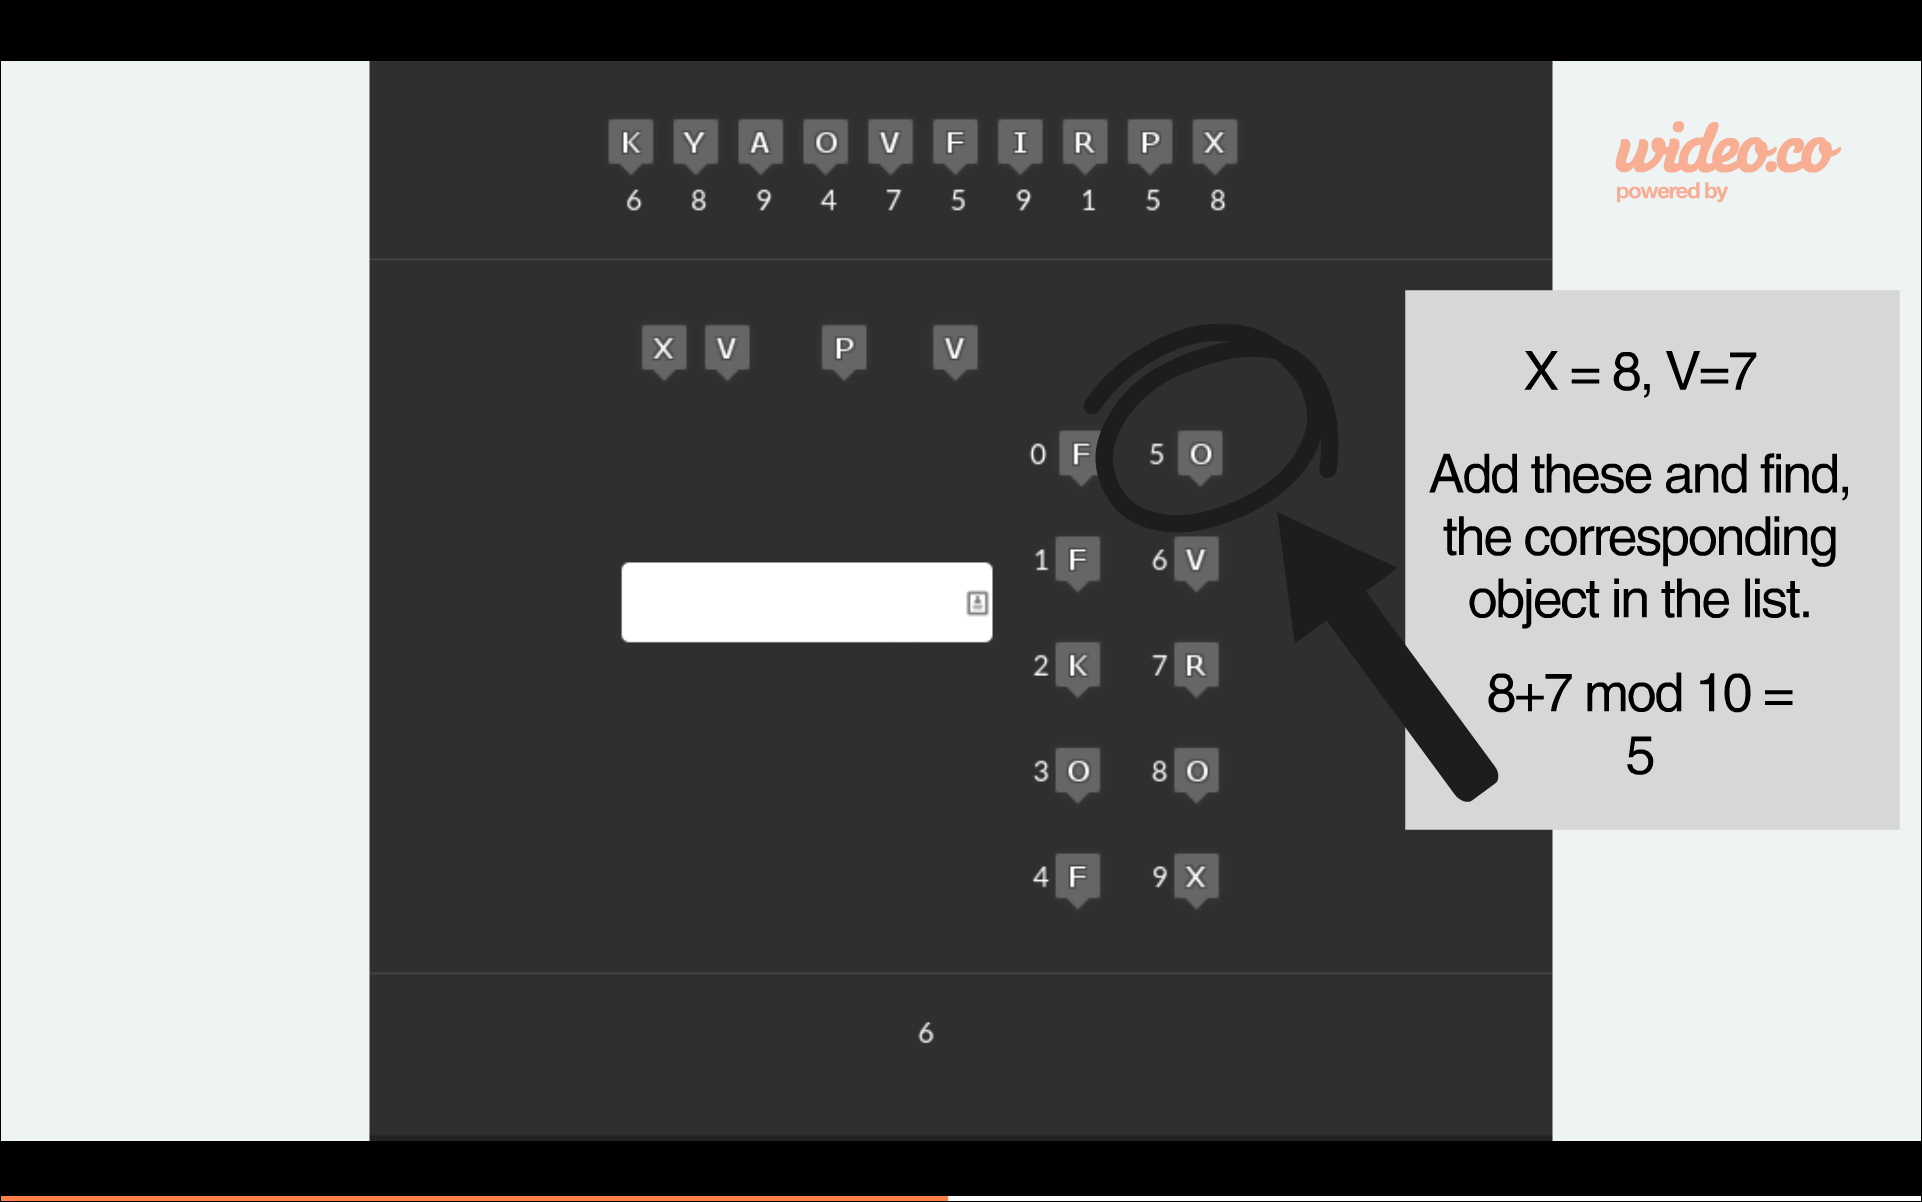
\includegraphics[width=\textwidth]{slides/slide3}
    \caption{Demo slide 3.}
    \label{slide3}
\end{figure}


\begin{figure}
    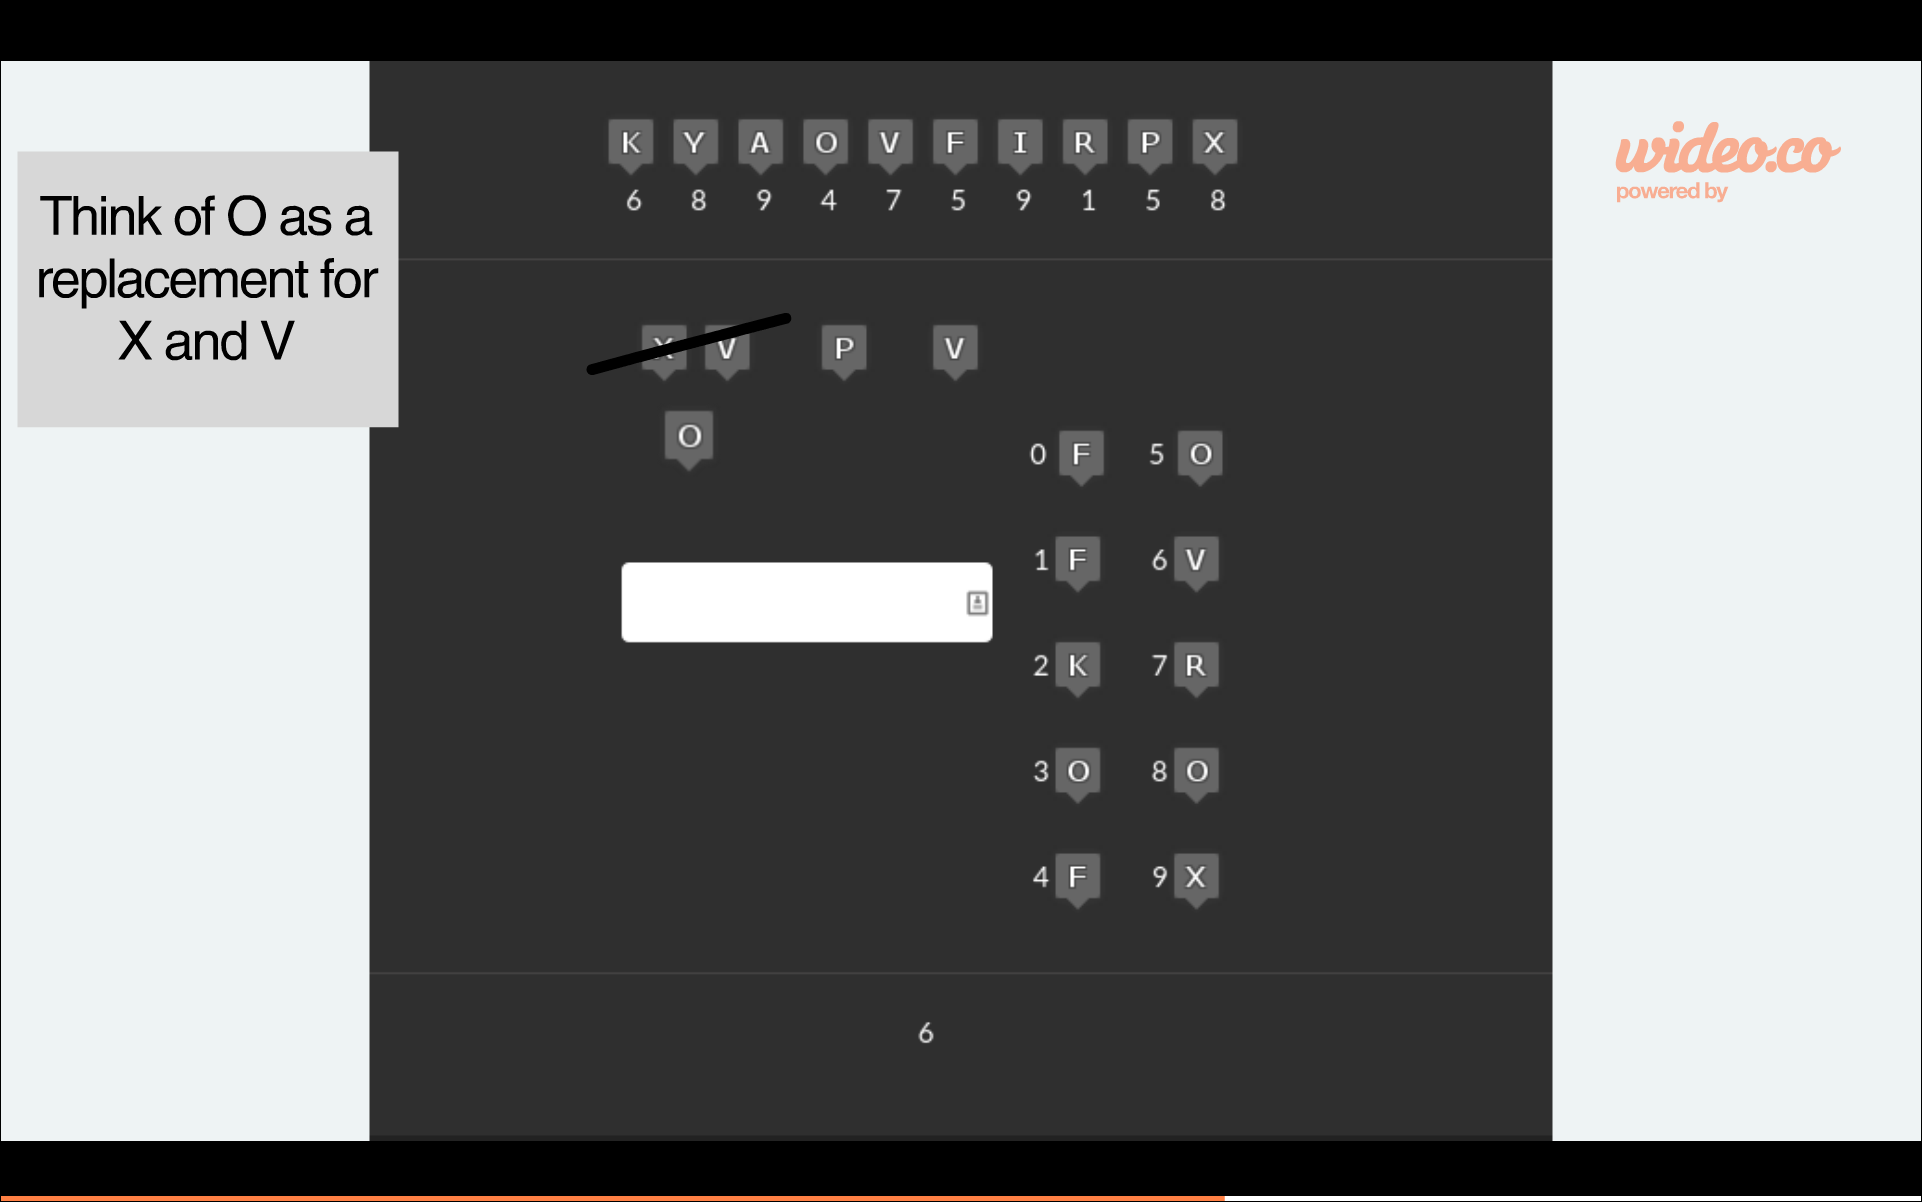
\includegraphics[width=\textwidth]{slides/slide4}
    \caption{Demo slide 4.}
    \label{slide4}
\end{figure}

\begin{figure}
    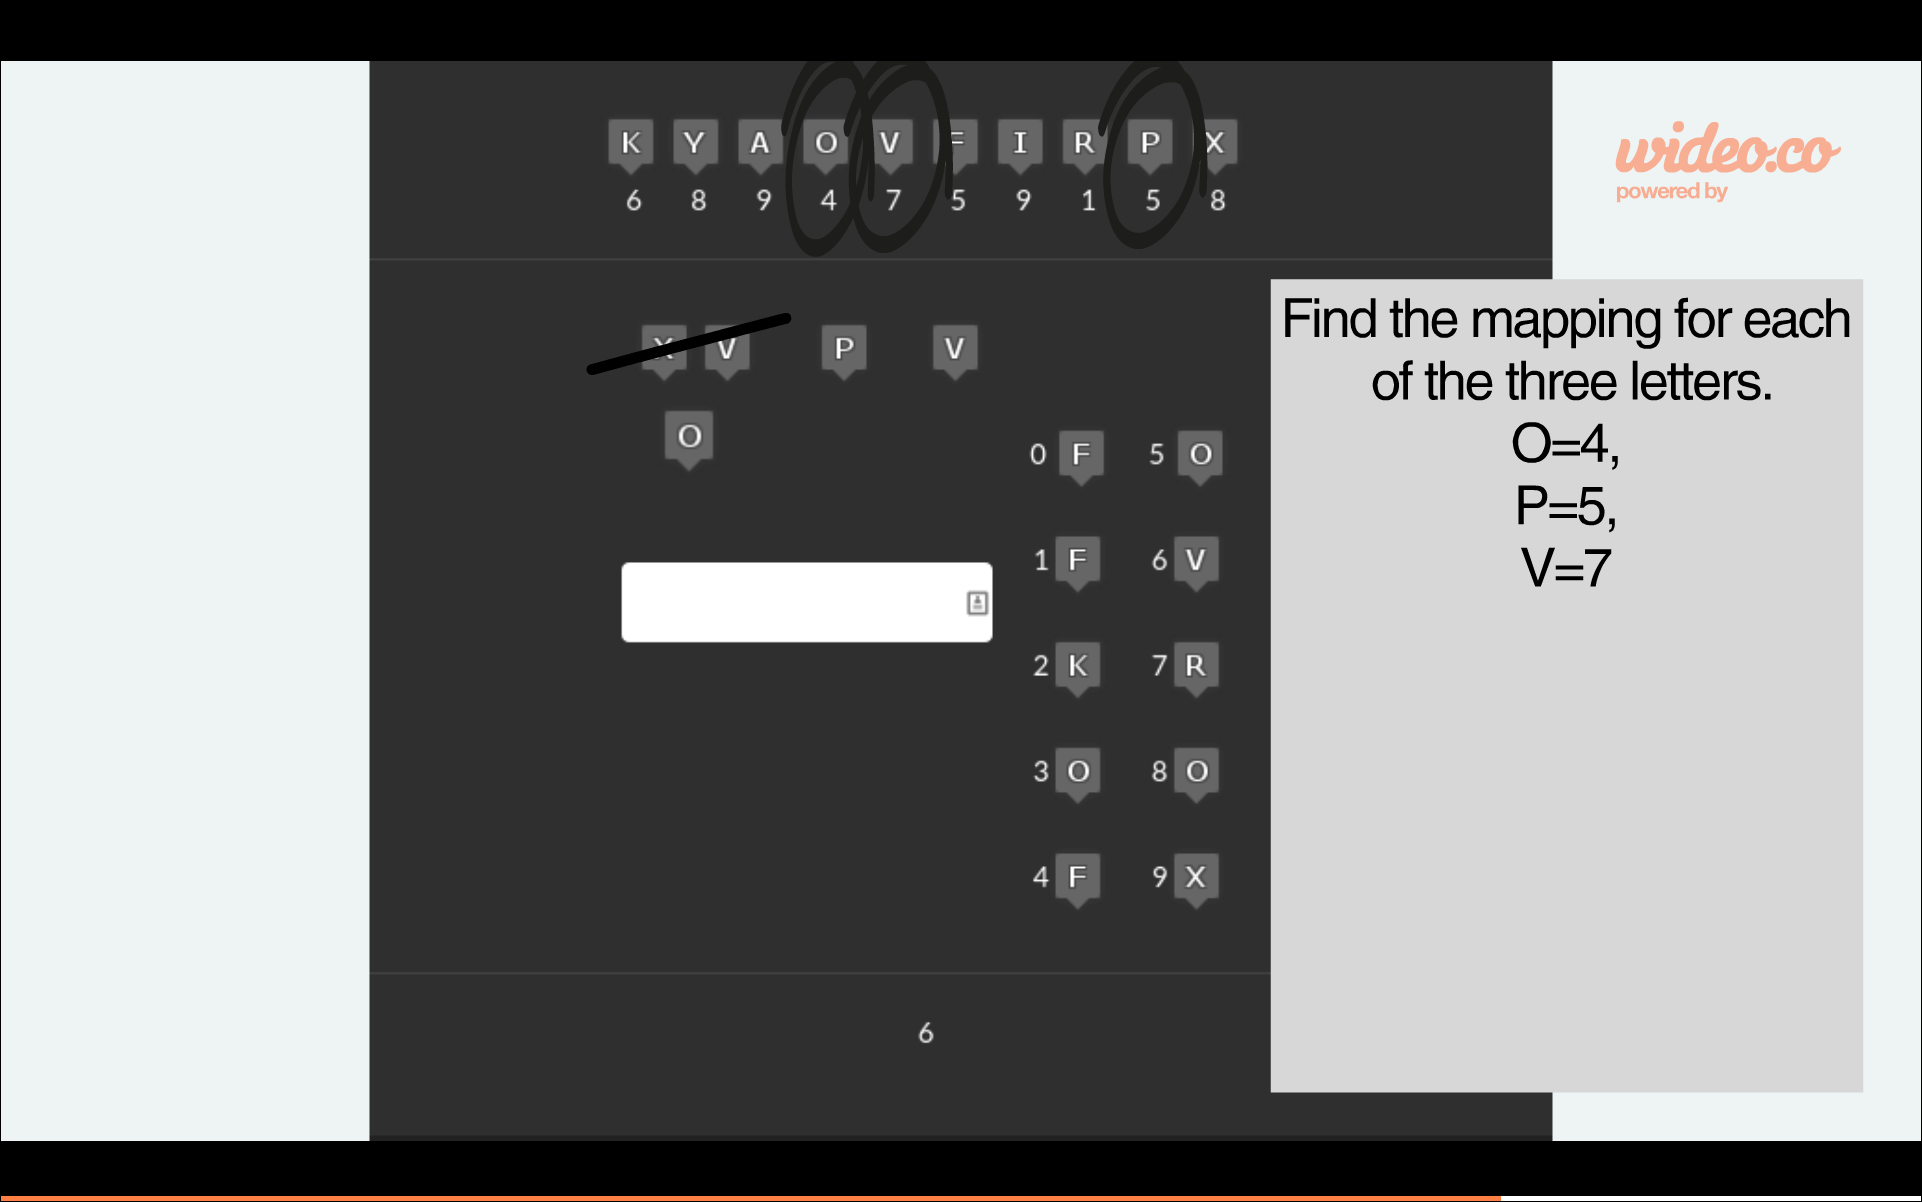
\includegraphics[width=\textwidth]{slides/slide5}
    \caption{Demo slide 5.}
    \label{slide5}
\end{figure}


\begin{figure}
    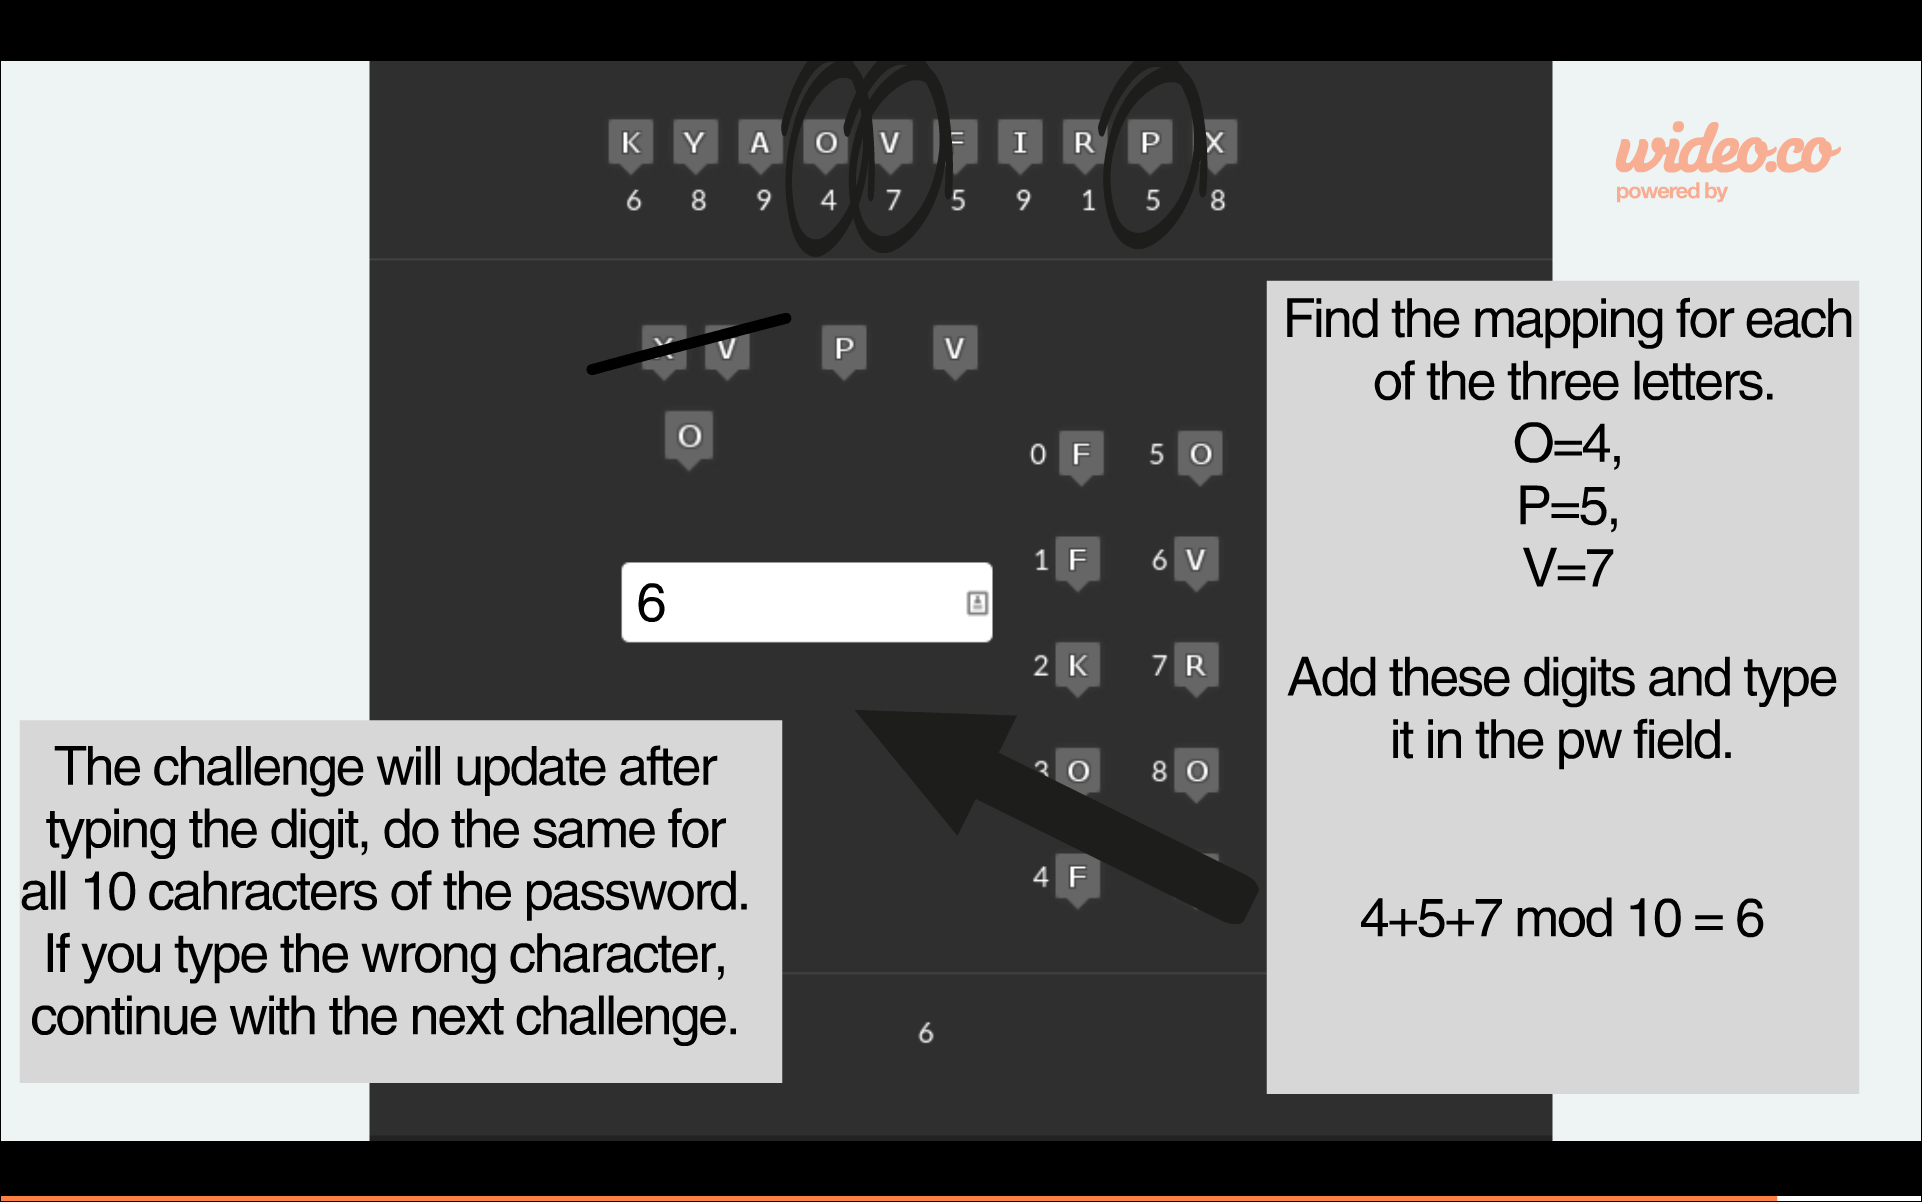
\includegraphics[width=\textwidth]{slides/slide6}
    \caption{Demo slide 6.}
    \label{slide6}
\end{figure}

\cleardoublepage
\chapter{Extension class files}\label{extension-classes}

\section{Content Script}\label{app:content-script}
\lstinputlisting[caption=Content script file., style=jsStyle, basicstyle=\scriptsize]{code/content_script.js}

The content script listens for the onload event triggered by the windows object when a new page is loaded. When receiving this event the updateUrl function(line 27) is called, which sends an update containing the \emph{window.location.hostname} which essentially is the hostname of the current page. Hostname is used since login forms may be located at different locations at different domains.
\par Next the script search the DOM for input fields of type "password" using the \emph{getPwdInputs} function(line 16). This function iterates through all the input fields looking for password fields. If a password field is found, an event listener is attached to the field, listening for events of type "input" which are sent when the field changes\footnote{https://developer.mozilla.org/en-US/docs/Web/API/EventTarget/addEventListener}. When the password field changes a message containing the new length of the password is sent to the controller. 

\section{Controller}\label{app:controller}
\lstinputlisting[caption=Angular controller., style=jsStyle, basicstyle=\scriptsize]{code/controllers.js}
The controller is responsible for all the business logic, keeping the storage updated with new users and new sites. The \emph{newSite} method on line 10 is called when then "new site"-button is clicked by the user, it then generates a new object of type Site with the domain name and selected site class( essentially the number of single digit challenges to be generated). The site is then added to the user object which is stored to the database to keep the storage persistent in case of disconnection. 
\par When the controller is loaded the first action executed is trying to load the user object from the storage (line 20), if no user object is found, the controller creates a new one. In the code presented here, a new user is initiated with a dummy site for demonstration purposes. All the storage specific methods are called from the \emph{chromeStorage} object, which makes it easy to do operations accessing the Chrome storage. The \emph{getOrElse} is used, which checks for a user object and creates a new if none is present. 
\par The controller also listens for messages from the content script, this event listener can be seen at line 62. When a message is received the \emph{handleMessage} is called to process the data, distinguishing between a changes in the URL and changes in password length. When data is received, the corresponding variable in the controller is updated. If a new site was added, the view is also updated, hiding the "new site"-button.

\section{App.js file}\label{app:app.js}
\lstinputlisting[caption=Angular launcher file., style=jsStyle, basicstyle=\scriptsize]{code/app.js}

The app.js file initiates the application, specifying the modules used as well as some helper functions, including get function responsible for generating the random challenges(line 66), note the argument \emph{siteclass} which contains the number of single digit challenges to be generated. 

\section{View file (partial file)}\label{app:view}
\lstinputlisting[caption=Angular view. Only included the table showing the challenges for readability., style=jsStyle, basicstyle=\scriptsize, firstline=12, lastline=91]{code/content.html}
The code shown in this listing contains the view where the challenges are presented, as well as the new site button and site classification radio buttons. Notice the \emph{ng-show} directive on line 14, this decides if the "new site"-functionality should be shown or not. If \emph{newSiteButton} is true it will appearer and vice versa, the same goes for the challenges which starts on line 34 with a similar directive, \emph{ng-hide}, which hides the challenges div if new site is visible.  
\par The challenges div is essentially a table containing a single digit challenge in each cell. Notice the double bracket notation, where each of the challenges are fetched. \emph{\{\{site.challenges[pw][i]\}\}} refers to the \emph{\$scope.site.challenges} which contains the challenges associated with the current active page. $pw$ is at any given time the length of the password field of the active web page, if $pw$ changes the challenges on display will automatically change through the two-way data binding in Angular. This way, the correct challenge will always be the one seen by the user.


\chapter{Experiment application}\label{experiment-views}

\begin{figure}
    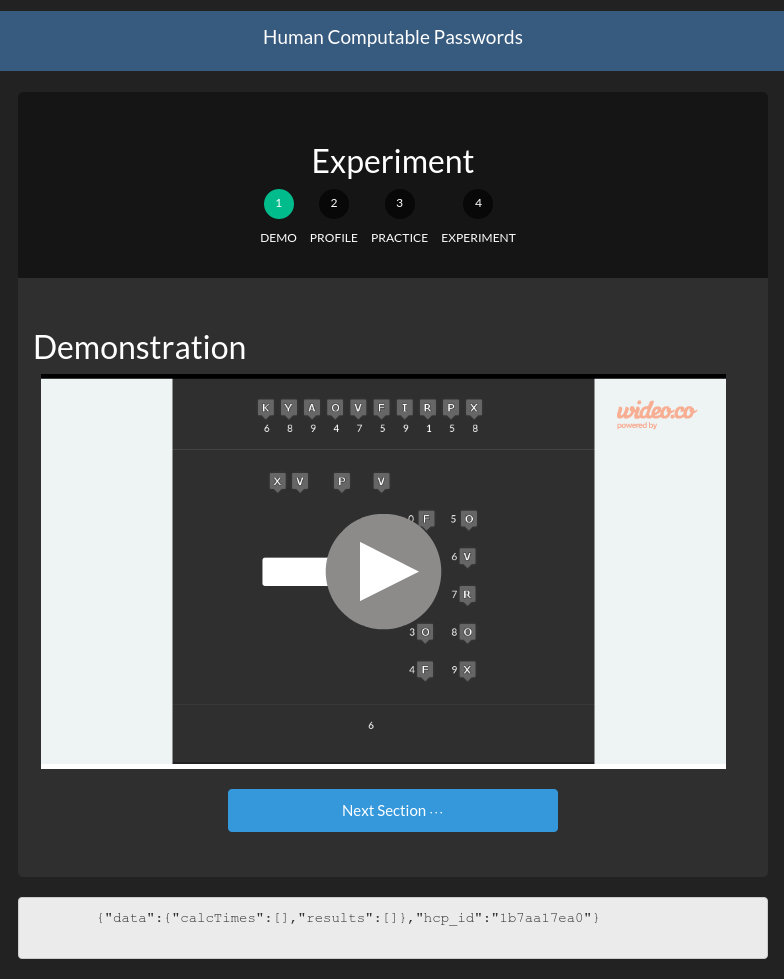
\includegraphics[width=\textwidth]{view1}
    \caption{First view shown to the user, containing a demonstration video. Created using \url{wideo.co}.}
    \label{view1}
\end{figure}

\begin{figure}
    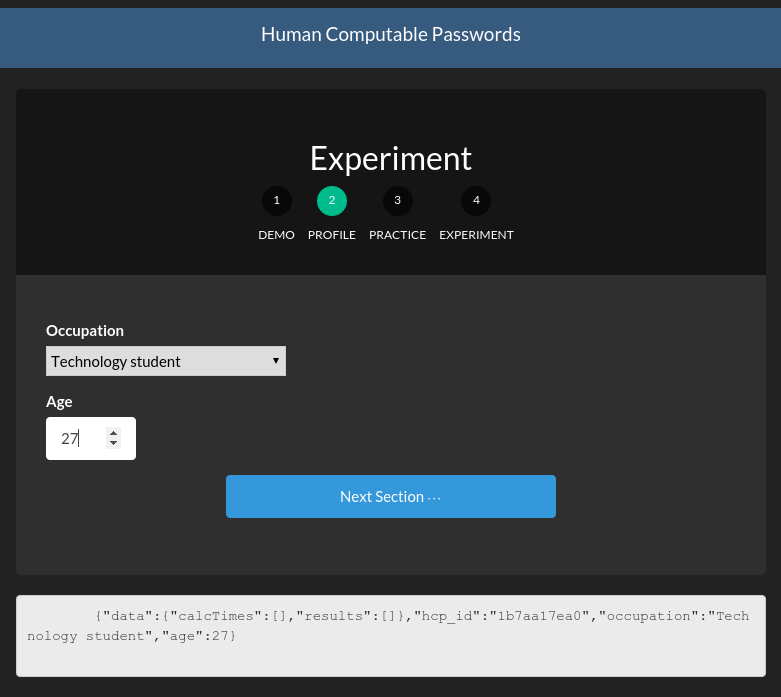
\includegraphics[width=\textwidth]{view2}
    \caption{Second view shown to the user, gathering some basic demographic data which might be relevant. }
    \label{view2}
\end{figure}

\begin{figure}
    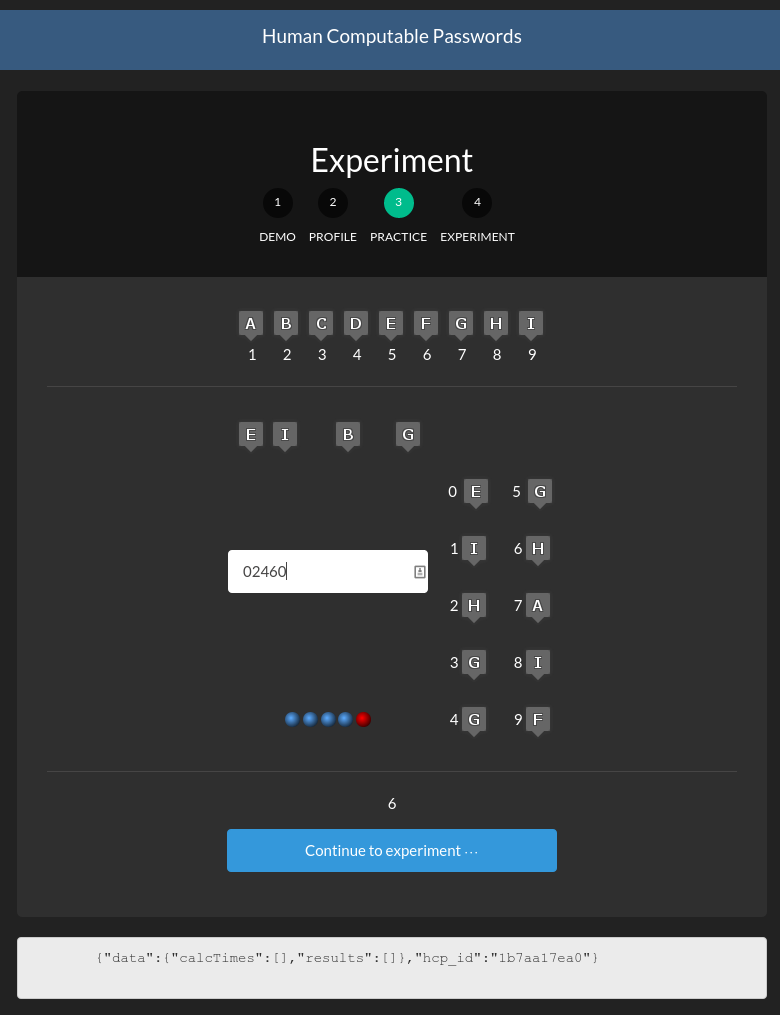
\includegraphics[width=\textwidth]{view3}
    \caption{Third view of the web application. Practice section used by the user before entering the actual experiment.}
    \label{view3}
\end{figure}

\begin{figure}
    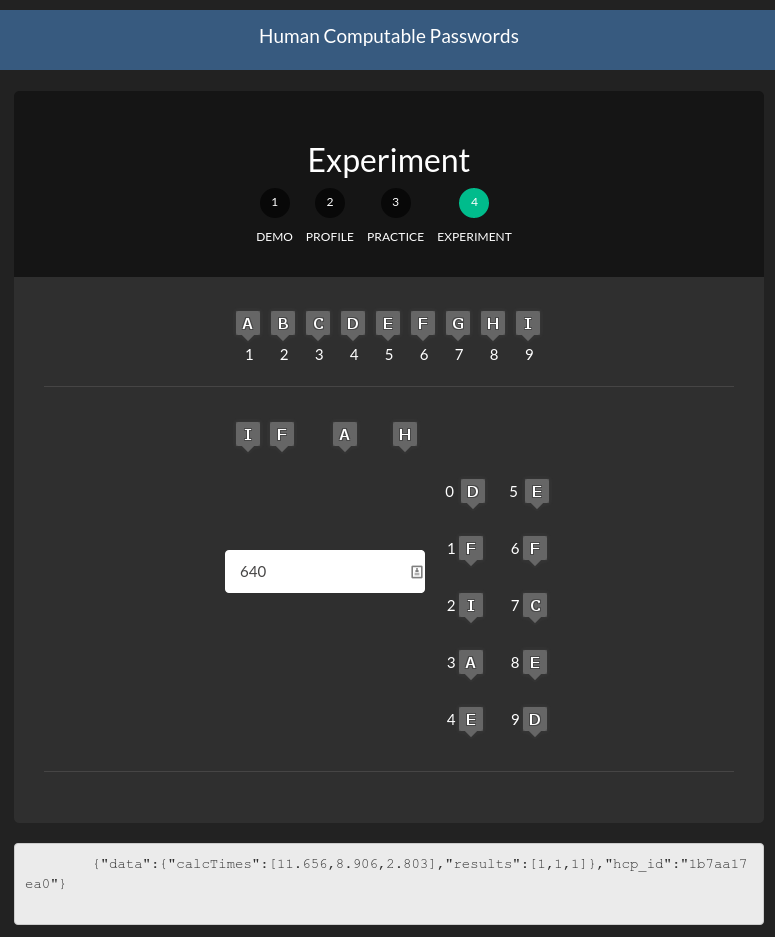
\includegraphics[width=\textwidth]{view4}
    \caption{Final view, containing the experiment form. The user will calculate the response to the challenge on display and enter the answer in the password field. When finished the results can be submitted. And eventually stored in the database.}
    \label{view4}
\end{figure}
